\chapter{Homographies}
\label{chapter:homography}






\section{Introduction}

%What is now a robust tool was not long ago a vibrant research topic. 



In \chap{\ref{chapter:geometry_homogeneous}} we discussed several types of geometric transformations of two-dimensional (2D) images: translations, rotations, skewing, scalings, and we saw that all could be modeled as the product between the coordinates of a point in the input image described using homogeneous coordinates and a $3 \times 3$ matrix.  Now that we have discussed camera models, we are well equipped to present a more general geometric image transformation that opens the door to many applications: the homography.

As we discussed in the previous \chap{\ref{chap:stereo_vision}}, if we capture a scene with two cameras from different viewpoints, corresponding points across both images are constrained by the epipolar constrain. In general, there is not a simple geometric transformation that maps pixels from one image into the pixels of the other image. To find that mapping we will need to know the three-dimensional (3D) location of each point as well as the relative camera translation and rotation between both images. %This means that if we want to transform one image into the other applying image warping (as described in section \ref{}), we need will need to know the 3D locations of all the points in the image. 

However, there are a few scenarios where we can find a simple transformation that allows warping one image into another image corresponding to a new camera location without requiring knowing the 3D scene structure: this will happen when the scene is planar (as in \fig{\ref{fig:illustration_homography}}) or when the two cameras are related just by a rotation (\fig{\ref{fig:rotation_homography}}). In those two cases the coordinates of corresponding points across the two images are related by a {\bf homography}.


\begin{figure}[h!]
    \centerline{
        \includegraphics[width=.455\linewidth]{figures/homography/IMG_7801_crop.jpg}
        ~~
        \includegraphics[width=.49\linewidth]{figures/homography/IMG_7802_crop.jpg}
    }
    \caption{These two images are (approximately) related by an homography.}
    \label{fig:illustration_homography}
\end{figure}

Homographies can be used in applications such as perspective correction, augmented reality, image stitching, creating bird's-eye views, correcting keystone distortions for projected images, and many others.

\marginnote{One popular tool available in many cameras and photography editing tools is the option to combine multiple overlapping images into a large panorama. The {\bf homography} is what is behind those tools.}

\section{Homography}

Let's start with a formal definition of the homography. A homography (or projective transformation) is a geometric transformation that preserves straight lines.
The homography is a function $h$ that maps points into points, $\mathbf{p}' = h(\mathbf{p})$, with the property that if points  $\mathbf{p}_1$, $\mathbf{p}_2$, and $\mathbf{p}_3$ are colinear, then the transformed points $h(\mathbf{p}_1)$, $h(\mathbf{p}_2)$, and $h(\mathbf{p}_3)$ are also colinear. Such a function,  $\mathbf{p}' = h(\mathbf{p})$, can be written in homogeneous coordinates as a product with a matrix:

\begin{equation}
    \begin{bmatrix}
        x' \\
        y' \\
        w'
    \end{bmatrix}
    =
    \begin{bmatrix}
        a & b & c \\
        d & e & f \\
        g & h & i
    \end{bmatrix}
    \begin{bmatrix}
        x \\
        y \\
        1
    \end{bmatrix}
    \label{eq:homography}
\end{equation}

This can be written in the short form:
\begin{equation}
    \mathbf{p}' = \mathbf{H} \mathbf{p}
    \label{eq:homography_generic}
\end{equation}
where $\mathbf{p}$ and $\mathbf{p}'$ correspond to 2D points in homogeneous coordinates, and $\mathbf{H}$ is a $3 \times 3$ matrix.

To prove that colinear points remain colinear after the homography we can use the equation of a line in homogeneous coordinates, $\boldsymbol{l}^\transpose \mathbf{p}=0$. From \eqn{\ref{eq:homography_generic}}, we have that $\mathbf{p} = \mathbf{H}^{-1} \mathbf{p}'$. Replacing the last equality into the equation of the line gives $(\mathbf{H} ^{-\transpose}\boldsymbol{l})^\transpose  \mathbf{p'}=0$, which corresponds to the equation of the line for the projected points $\mathbf{p}'$.


%We can rewrite this expression as  $\boldsymbol{l}^T (\mathbf{H} ^{-1}\mathbf{H} ) \mathbf{p}=0$. Using eq.~\ref{eq:homography_generic}, we can rewrite the last expression as $(\mathbf{H} ^{-T}\boldsymbol{l})^T  \mathbf{p'}=0$, which corresponds to the equation of the line for the projected points $\mathbf{p}'$. 

In a general homography, angles and lengths are not preserved. Therefore, parallel lines might not remain parallel, and lines of identical length might have different lengths after a homography.  \Fig{\ref{fig:illustration_homography2}} shows how a planar grid gets transformed after applying a homography.

\begin{figure}[h!]
    \centerline{
        \includegraphics[width=.7\linewidth]{figures/homography/example_homography.eps}
    }
    \caption{Homography. Colinear points remain colinear after transformation. Angles between lines are not preserved.}
    \label{fig:illustration_homography2}
\end{figure}




Let's start discussing in which scenarios the coordinates of points between to images are related by a homography.


\subsection{Camera Rotation}
Consider the following three images shown in \fig{\ref{fig:example_three_images}}.


\begin{figure}[h!]
    \centerline{
        \includegraphics[width=0.445\linewidth]{figures/homography/3_IMG_7883_small.jpg}
        ~~\includegraphics[width=0.25\linewidth]{figures/homography/2_IMG_7884_small.jpg}
        ~~\includegraphics[width=0.25\linewidth]{figures/homography/1_IMG_7885_small.jpg}
    }
    \caption{Three pictures taken by rotating the camera while trying to keep the camera center fixed.}
    \label{fig:example_three_images}
\end{figure}


The three images are taken from the same point by rotating the camera. There is no translation between the three camera positions as the photographer took the three images by keeping the camera origin static when moving the camera. Under this condition, the coordinates of the corresponding points across each pair of images are related by a homography independently of how far they are from the camera.

Here, we show that the mapping between feature point locations in two cameras differing only in their 3D orientation, as shown in \fig{\ref{fig:rotation_homography}}, is a $3\times3$ matrix transformation of their 2D positions written in homogeneous coordinates, that is, a homography.


\begin{figure}[h!]
    \centerline{
        \includegraphics[width=1\linewidth]{figures/homography/rotation_homography_vs3.eps}
    }
    \caption{Camera rotation generates two images related by a homography.}
    \label{fig:rotation_homography}
\end{figure}

We start by setting the world coordinate system aligned with the coordinate system of camera 1, as shown in \fig{\ref{fig:rotation_homography}}.  Therefore, the projection of a 3D point, $\mathbf{P}=[X,Y,Z]^\transpose$, into the camera 1 plane gives, setting the translation vector to be zero:
\begin{equation}
    \lambda_1
    \begin{bmatrix}
        x \\
        y \\
        1
    \end{bmatrix}
    =
    \mathbf{K}
    \begin{bmatrix}
        \mathbf{I} & \mathbf{0}
    \end{bmatrix}
    \begin{bmatrix}
        X \\
        Y \\
        Z \\
        1
    \end{bmatrix}
    =
    \mathbf{K}
    \begin{bmatrix}
        X \\
        Y \\
        Z
    \end{bmatrix}
    \label{eq:projectionintofirstcamera}
\end{equation}

We can now project the same 3D point into camera 2. Setting the translation vector to be zero in \eqn{\ref{eq:combinedexpandedsmaller}}, and writing the $3\times3$ rotation matrices for camera 2 as $\mathbf{R}$, we have for the observed position of a common 3D point observed from camera 2:


\begin{equation}
    \lambda_2
    \begin{bmatrix}
        x' \\
        y' \\
        1
    \end{bmatrix}
    =
    \mathbf{K}
    \begin{bmatrix}
        \mathbf{R} & \mathbf{0}
    \end{bmatrix}
    \begin{bmatrix}
        X \\
        Y \\
        Z \\
        1
    \end{bmatrix}
    =
    \mathbf{K}  \mathbf{R}
    \begin{bmatrix}
        X \\
        Y \\
        Z
    \end{bmatrix}
    \label{eq:projectionintosecondcamera}
\end{equation}

As both cameras see the same 3D point, $\mathbf{P}=[X,Y,Z]^\transpose$, we can invert the two projection equations (\ref{eq:projectionintofirstcamera}) and (\ref{eq:projectionintosecondcamera}) to get the following relationship:


\begin{equation}
    \begin{bmatrix}
        X \\
        Y \\
        Z
    \end{bmatrix}
    =
    \lambda_1 \mathbf{K}^{-1}
    \begin{bmatrix}
        x \\
        y \\
        1
    \end{bmatrix}
    =
    \lambda_2 \mathbf{R}^{-1} \mathbf{K}^{-1}
    \begin{bmatrix}
        x' \\
        y' \\
        1
    \end{bmatrix}
    \label{eq:inverted_projectionintofirstcamera}
\end{equation}

\marginnote{Observe that \eqn{\ref{eq:inverted_projectionintofirstcamera}} does not mean that we can recover the 3D coordinates of a point from the image coordinates. We know that this is impossible, so what is the issue? The subtlety is that the equations are written as functions of $\lambda_1$ and $\lambda_2$, which we do not know when only given image coordinates. Therefore, the equations only specify the equation of a ray when looking at all possible values of $\lambda_1/\lambda_2$. }

Using the last equality, we can establish the following relationship between the corresponding image points, in homogeneous coordinates:
%\begin{equation}
%  \lambda_1 \left [
%   \begin{array}{c}
%   x \\
%    y \\
%    1
%    \end{array}
%    \right ] 
%    =
%    \lambda_2 
%    \mathbf{K} \mathbf{R}^{-1} \mathbf{K}^{-1} 
%    \left [
%    \begin{array}{c}
%    x' \\
%    y' \\
%    1
%    \end{array}
%    \right ]     
%    \label{eq:intermediate_step}
%\end{equation}

\begin{equation}
    \lambda_2 / \lambda_1
    \begin{bmatrix}
        x' \\
        y' \\
        1
    \end{bmatrix}
    =
    \mathbf{K} \mathbf{R} \mathbf{K}^{-1}
    \begin{bmatrix}
        x' \\
        y' \\
        1
    \end{bmatrix}
    \label{eq:homo3}
\end{equation}


%in this last equation,  $\lambda_2$ can be set to 1 as a scaling of all the coordinates has no effect on the homogeneous coordinates.  On the other hand $\lambda_1$ can not be set to 1 as it is constrained to be different than 1 by the equation \ref{eq:intermediate_step}.

We can write the relationship between corresponding points as
\begin{equation}
    \lambda
    \begin{bmatrix}
        x' \\
        y' \\
        1
    \end{bmatrix}
    =
    \mathbf{H}
    \begin{bmatrix}
        x \\
        y \\
        1
    \end{bmatrix}
\end{equation}
where $\mathbf{H}$ is a $3\times3$  matrix.  Thus, camera rotation modifies the locations of the image points by a homography. The relationship also holds if the two cameras have different intrinsic camera parameters. This concludes the proof.

%Thus, an additional transformation to add to the 2D transformations of Section~\ref{sect:2dtransforms} is a homography, given by a general $3\times3$ matrix transformation of homographic coordinates:
%\begin{equation}
%    \mathbf{H} =             
%    \left [
%    \begin{array}{ccc}
%    a & b & c \\
%    d & e & f \\
%    g & h & i
%    \end{array}
%    \right ]
%\end{equation}

Under certain conditions, a homography predicts the position of points when viewed with another camera from another position. We just discussed one condition, when the two cameras differ in their position by a rotation about a common center of projection.  We will now consider another case.

\subsection{Planar Surface}

A second case is when two cameras observe a 2D plane \cite{Hartley2004}. In that case, the coordinates of corresponding points across the two camera views, for points inside the plane, are related by a homography (\fig{\ref{fig:example_two_images_facade}}).




\begin{figure}
    \centerline{
        \includegraphics[width=0.45\linewidth]{figures/homography/IMG_7127_crop.jpg}
        ~~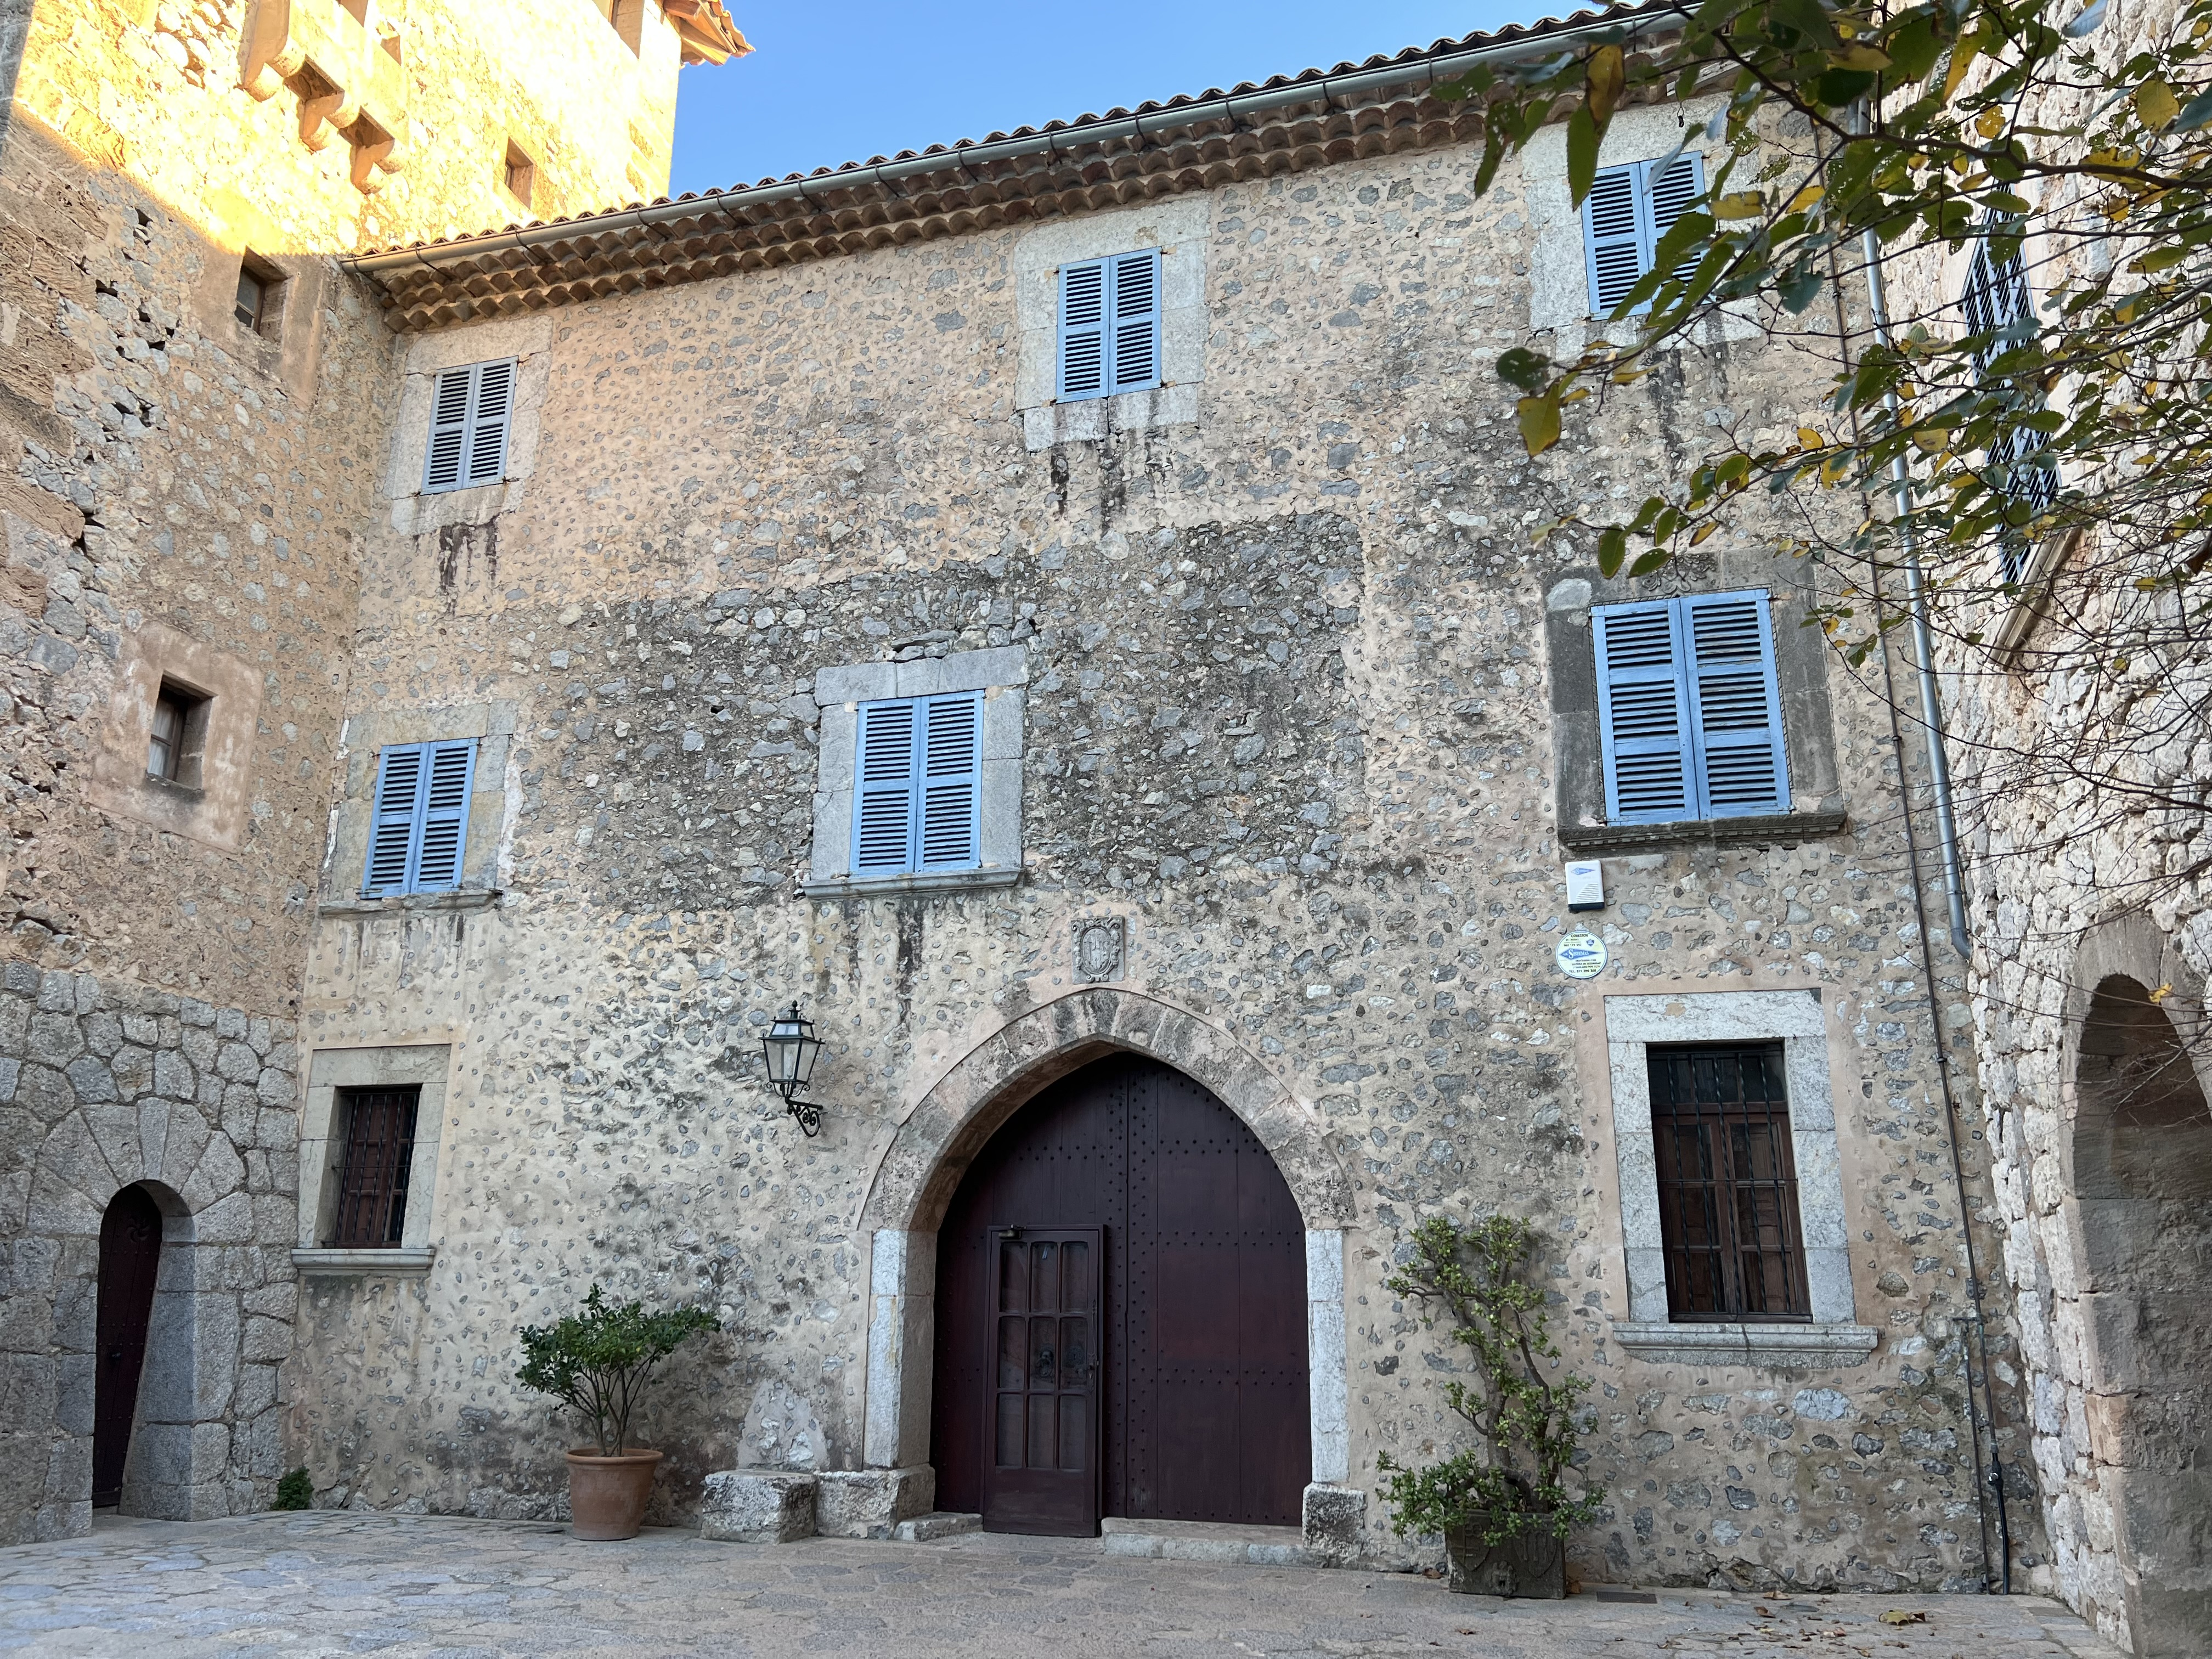
\includegraphics[width=0.45\linewidth]{figures/homography/IMG_7126.jpg}
    }
    \caption{Two pictures of a building facade taken from different positions. The coordinates of corresponding points on the planar facade are related by a homography.}
    \label{fig:example_two_images_facade}
\end{figure}


To prove this, we can first show that the coordinates inside a plane relate to the coordinates in the image plane by a homography independently of relative position between the plane and the camera. Therefore, the relationship between points across two images will also be related by a homography.

%\begin{figure}[h!]
%\centerline{
%\includegraphics[width=0.7\linewidth]{figures/homography/planar_scene.eps}
%}
%\caption{Planar scene seeing by two cameras. The coordinates of points on the plane (using ) are related by an homography to the coordinates on the image planes of both cameras.}
%\label{fig:planar_homography}
%\end{figure}


We start by placing the world-coordinate system on the plane so that the plane is defined by $Z=0$ as shown in the \fig{\ref{fig:homography_plane_geometry}}. Note that the origin can be placed at any arbitrary location in the world.


\begin{figure}
    \centerline{
        \includegraphics[width=0.7\linewidth]{figures/homography/homography_plane_geometry2.eps}
    }
    \caption{Geometry of a the projection of a planar scene. The origin of the world-coordinates system is placed inside the plane and the $Z$-axis is perpendicular to it.}
    \label{fig:homography_plane_geometry}
\end{figure}

% Slide 22 in: http://www.cs.columbia.edu/~allen/F17/NOTES/homography_pka.pdf
The proof is similar to what we did in the previous section. We start writing the projection equation
\begin{equation}
    \lambda
    \begin{bmatrix}
        x \\
        y \\
        1
    \end{bmatrix}
    =
    \mathbf{K}
    \begin{bmatrix}
        \mathbf{R} & \mathbf{t}
    \end{bmatrix}
    \begin{bmatrix}
        X \\
        Y \\
        Z \\
        1
    \end{bmatrix}
\end{equation}

Note that we are not using the same notation for the translation vector as we used in \eqn{\ref{eq:extrinsic}}. You can obtain the same by setting $\mathbf{t}= -\mathbf{R} \mathbf{T}$, where $ \mathbf{R}$ and $\mathbf{T}$ are the translation and rotation of the camera with respect to the world-coordinate system. As we can put the world-coordinate system in any arbitrary location, we chose the world-coordinates system to be so that points in the plane have coordinates $Z=0$ as shown in \fig{\ref{fig:homography_plane_geometry}}. Therefore, we can write:
\begin{equation}
    \lambda
    \begin{bmatrix}
        x \\
        y \\
        1
    \end{bmatrix}
    =
    \mathbf{K}
    \begin{bmatrix}
        \mathbf{R} & \mathbf{t}
    \end{bmatrix}
    \begin{bmatrix}
        X \\
        Y \\
        0 \\
        1
    \end{bmatrix}
    =
    \mathbf{K}
    \begin{bmatrix}
        \mathbf{c}_1 & \mathbf{c}_2 & \mathbf{t}
    \end{bmatrix}
    \begin{bmatrix}
        X_1 \\
        Y_1 \\
        1
    \end{bmatrix}
\end{equation}
Where $c_i$ is the column $i$ of the rotation matrix $\mathbf{R}$. As the last expression contains the product of two $3 \times 3$ matrices, we can write
\begin{equation}
    \lambda
    \begin{bmatrix}
        x \\
        y \\
        1
    \end{bmatrix}
    =
    \mathbf{H}
    \begin{bmatrix}
        X \\
        Y \\
        1
    \end{bmatrix}
    \label{eq:projectionintofirstcamera}
\end{equation}
This last result shows that the coordinates of points on the plane are related to the corresponding points in the image plane by a homography.

As \eqn{\ref{eq:projectionintofirstcamera}} is true for any camera, the relationship between corresponding points in the two cameras will also be related by a homography when the points correspond to points in a plane in the 3D space. \marginnote{A homography is a stronger constraint than the epipolar constraint between corresponding points across two camera views. However, the homography only applies under certain conditions as we have seen, while the epipolar constraint always holds. }


\section{Creating Image Panoramas}


Let's now study a popular application of the homography: stitching images to create large panoramas. To create a large panorama from multiple pictures, the images need to be taken by a rotating camera without translation.

To stitch together images, one needs to estimate the homography relating the images to be stitched together.  While one could estimate the rotation and intrinsic camera matrices within \eqn{\ref{eq:homo3}} to compute the homography, it is usually simpler to follow the procedure below.

%Before exploring a few applications of the homography, lets study how to estimate the parameters of the homography relating corresponding points between two images. 

We will start assuming we have some initial correspondences between each pair of images as shown in \fig{\ref{fig:fig_matching_two_images}}. The correspondences in this example are computer using {\bf speeded up robust features} (SURF) \cite{Bay2008346}. \index{SURF}
%[1] Bay, H., A. Ess, T. Tuytelaars, and L. Van Gool. “SURF:Speeded Up Robust Features.” Computer Vision and Image Understanding (CVIU).Vol. 110, No. 3, pp. 346–359, 2008.


\begin{figure}[h!]
    \centerline{
        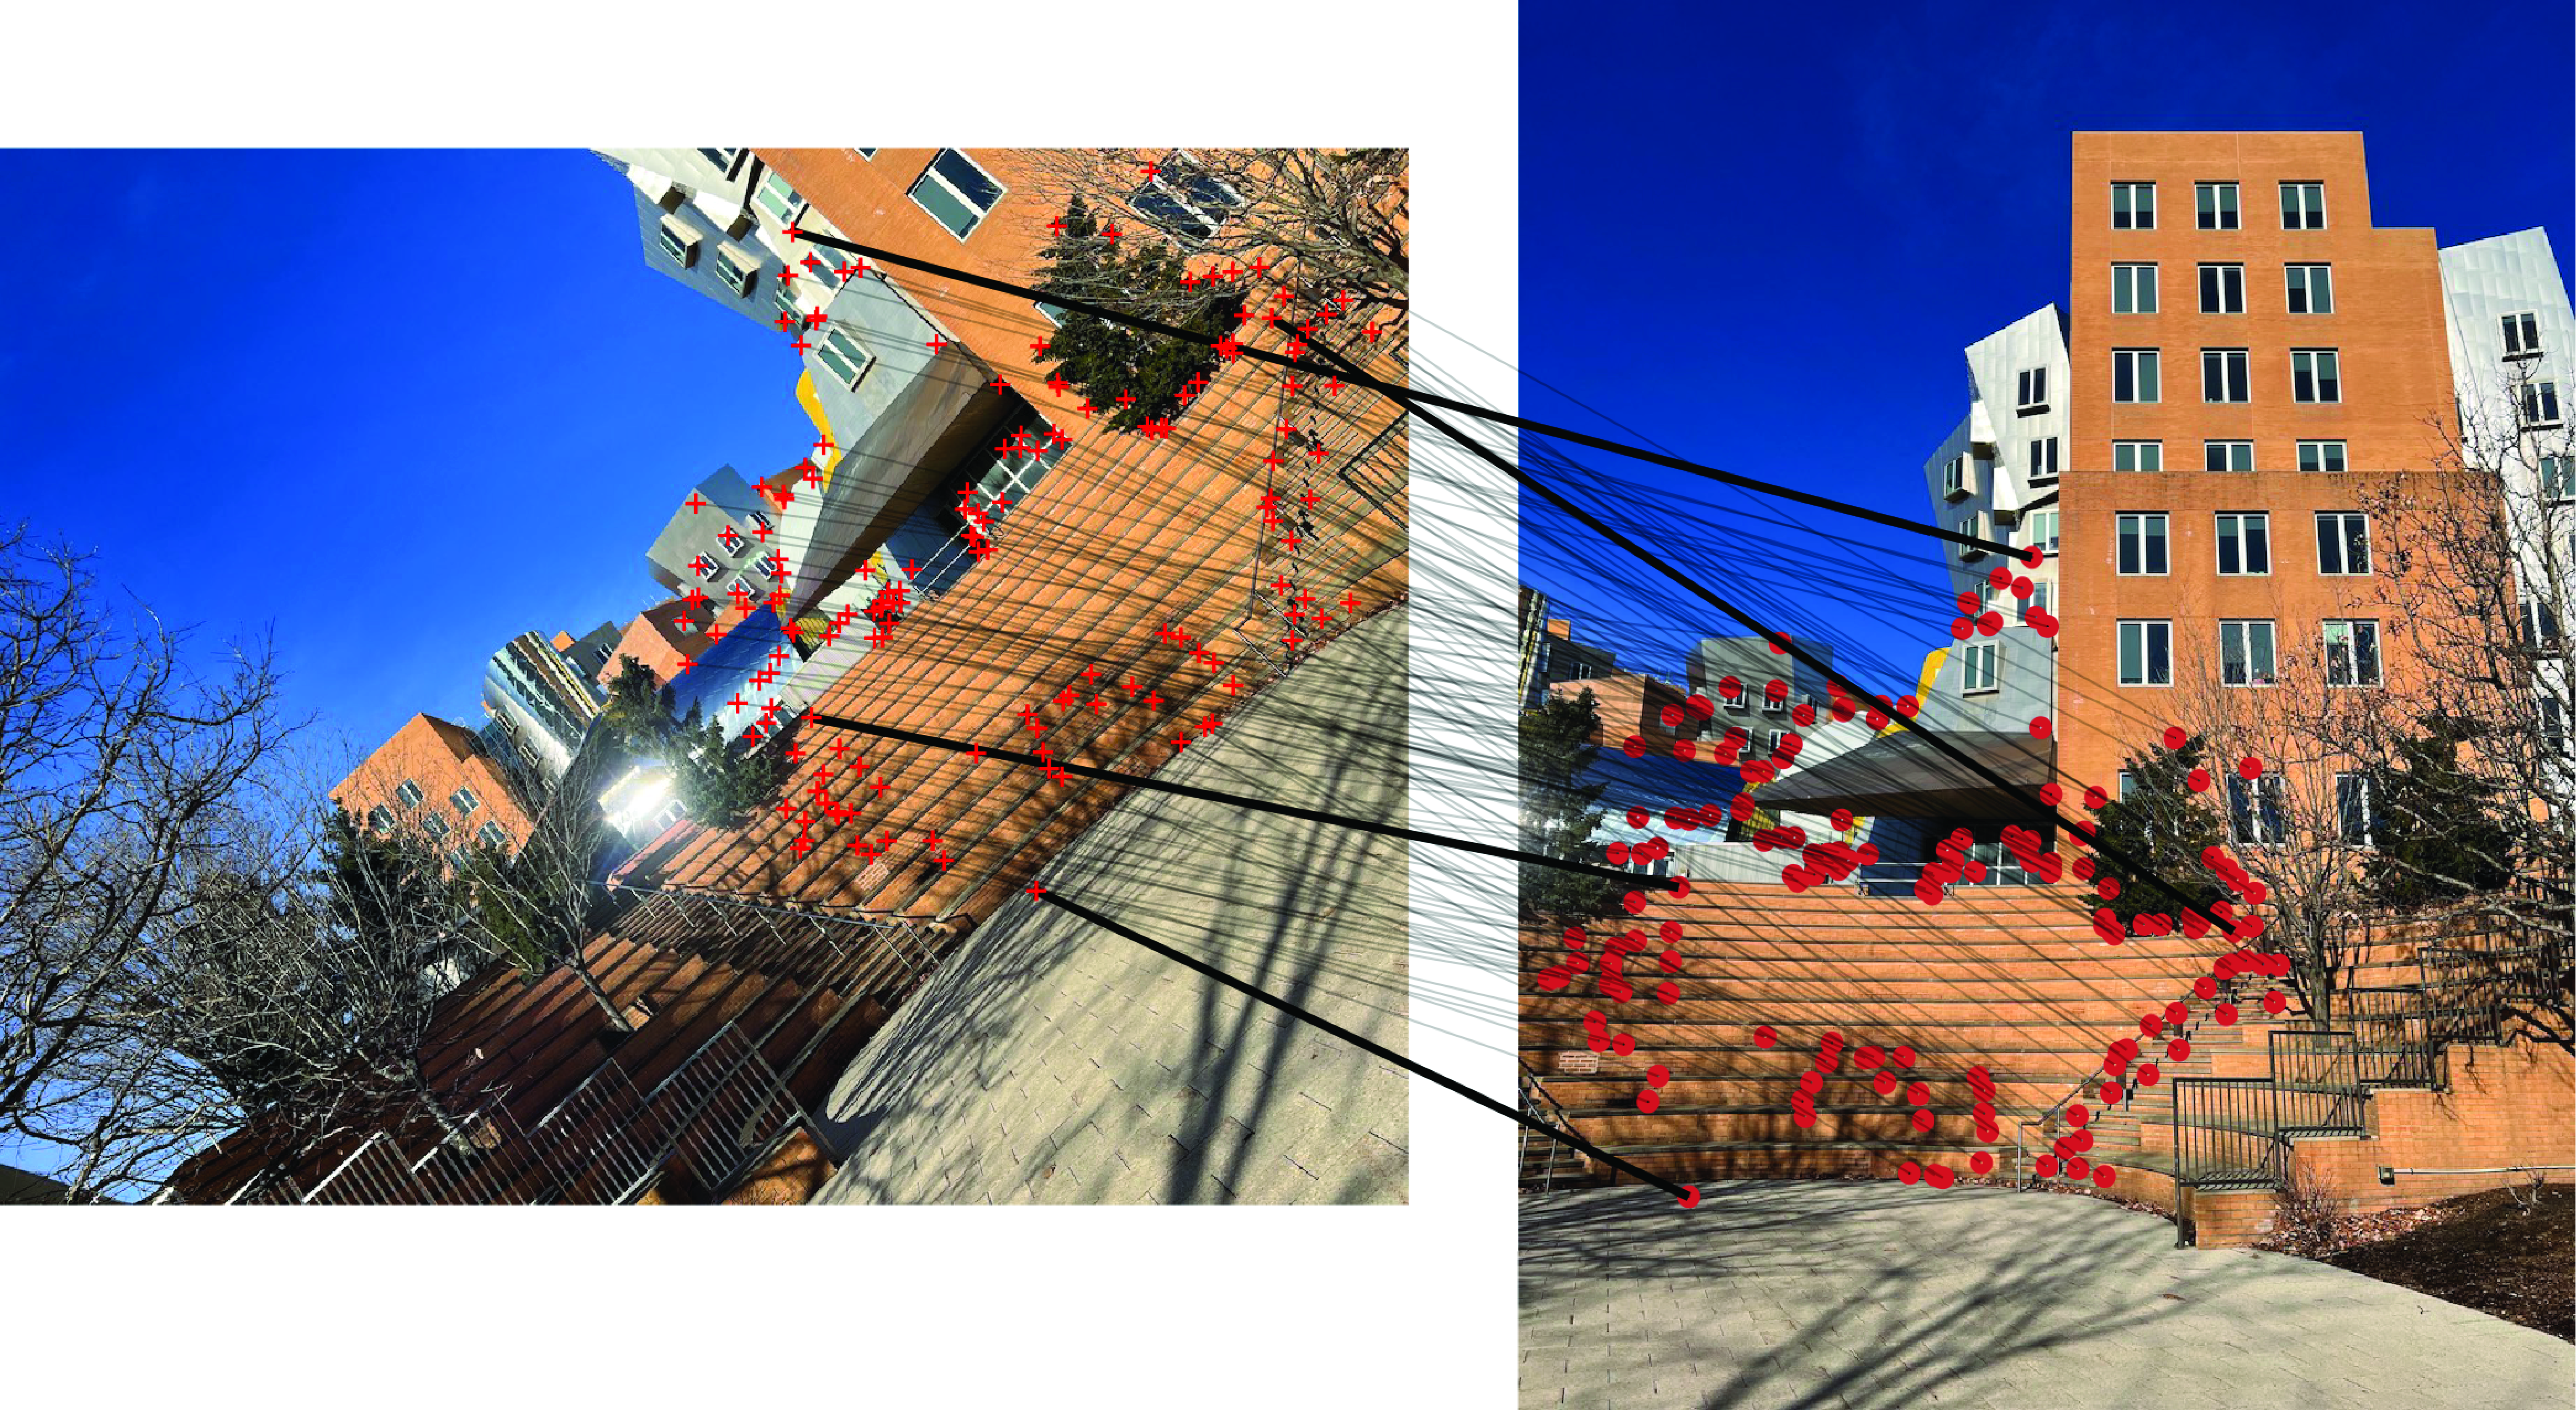
\includegraphics[width=1\linewidth]{figures/homography/fig_matching_two_images3.eps}
    }
    \caption{Two overlapping images and some found correspondences using SURF descriptors. A random set of four correspondences are highlighted.}
    \label{fig:fig_matching_two_images}
\end{figure}

\subsection{Direct Linear Transform Algorithm}

Given a set of point locations, and their correspondences across the two cameras, we can compute the homography relating the locations of imaged points within the two cameras.  To estimate the homography we can use the direct linear transform (DLT) algorithm, as we did for the camera calibration problem in section \ref{sec:camera_calibration}. This will give us a linear set of equations for the parameters of the homography matrix with the form:
\begin{equation}
    \mathbf{A} \mathbf{h} = \mathbf{0}
\end{equation}
where $\mathbf{A}$ is a $2N \times 9$ matrix, when given $N$ corresponding pairs. The vector $\mathbf{h}$ contains all the elements of the matrix $\mathbf{H}$ stacked as a column vector of length 9. Note that $\mathbf{h}$ only has 8 degrees of freedom as the results do not change for a global scaling of all the values. Therefore we will need at least four correspondences to estimate the homography between two sets of corresponding points, as the ones shown in \fig{\ref{fig:fig_matching_two_images}}. As before, the solution is the vector that minimizes the residual $\|\mathbf{A} \mathbf{h} \|^2$. The result is given by the eigenvector of the matrix $\mathbf{A}^\transpose \mathbf{A}$ with the smallest eigenvalue.

In practice, to get accurate results, it is useful to also minimize the reprojection error after you initialize with the DLT solution since $\|\mathbf{A} \mathbf{h} \|^2$ is meaningless geometrically.


%Consider the $i$th pair of feature point locations, rendered at position $[x,y,w]'$ in homogeneous coordinates in the first camera and at position $[x',y',w']'$ in the second.  Because the two homogeneous coordinate vectors, and the homography relating them, are all defined only to within a multiplicative constant, without loss of generality, we can set $w=1$.  Then we have, for the $i$th matching feature points,
%\begin{equation}
%              \left [
%    \begin{array}{c}
%    x_i' \\
%    y_i' \\
%    w_i' 
%    \end{array}
%    \right ]   
%    =
%    \left [
%    \begin{array}{ccc}
%    a & b & c \\
%    d & e & f \\
%    g & h & i
%    \end{array}
%    \right ]
%    \left [
%    \begin{array}{c}
%    x_i \\
%    y_i \\
%    1 
%    \end{array}
%        \right ] 
%        \label{eq:homo1}
%\end{equation}
%
%Converting Eq.~(\ref{eq:homo1}) to heterogeneous coordinates yields the constraint,
%\begin{eqnarray}
%        x_i' & = & \frac{a x_i + b y_i + c}{g x_i + h y_i + i} \\
%        y_i' & = & \frac{d x_i + e y_i + f}{g x_i + h y_i + i} 
%\end{eqnarray}
%Rearranging terms, we have these two constraints from the $i$ feature point pair:
%\begin{eqnarray}
%        g x_i x_i' +  h y_i x_i' + i x_i' -a x_i - b y_i - c  = 0 \\
%           \label{eq:constraints1}
%        g x_i y_i' +  h y_i y_i' + i x_i' -d x_i - e y_i - f = 0
%        \label{eq:constraints2}
%\end{eqnarray}
%The equations Eq.~(\ref{eq:constraints1}) and Eq.~(\ref{eq:constraints2}) above, for all $i = 1 \ldots N$, where $N$ is the number of feature point pairs can be written compactly in matrix form,
%\begin{equation}
%    \mathbf{A} \mathbf{h} = 0
%    \label{eq:homogeneous}
%\end{equation}
%where $\mathbf{h}$ contains the terms $a, b, \ldots, i$ stacked into a vector.  This homogeneous least squares problem can be solved for the unit norm values of the best-fitting homography matrix parameters (stacked into the vector elements of $\mathbf{h}$) by finding the right singular vector corresponding to the smallest singular value of the matrix, $\mathbf{A}$ \cite{Forsyth2012}.  That 9-component singular vector specifies the homography transformation relating the positions in the first camera image to the positions in the second.


\subsection{Robust Model Fitting: Random Sampling with Consensus}
\label{sec:RANSAC}

To perform the image stitching in the section above, we had to find the homography parameters that best described the transformation from one image to another. Because the detection of the feature points can be noisy, the homography fitting needs to be robust against inevitable feature mismatches between images.  A good algorithm to fit models to data robustly is  RANSAC \cite{Fischler1981}, which stands for {\bf random sampling with concensus}. \index{RANSAC}
\marginnote{RANSAC, introduced in 1981 by Fischler and Bolles \cite{Fischler1981}, has been a workhorse in computer vision ever since \cite{Zisserman2006}.}

The procedure for RANSAC is simple, and the name contains most of the steps of the algorithm.  First, randomly select a sufficient set of datapoints to fit the parameters of some model.  The could be the parameters that define a line, some other structure, or a homography.  Then, compute the model parameters from the randomly sampled set of points. Compute the inliers in the dataset, that is, the datapoints that fit the model (or achieve consensus) to within some tolerance.  Repeat that procedure some number of times, $N$.    Compute a final model from the set of inlier points corresponding to the largest number of inlier datapoints.

\Fig{\ref{fig:ransac}} shows a simple instantiation of this algorithm for the case of robustly fitting a straight line model to a collection of datapoints (\fig{\ref{fig:ransac}}[a]).  First, a number of datapoints, sufficient to uniquely specify the model parameters, are drawn from the dataset.  For this problem, that is two points.  Two randomly selected points are marked in green in \fig{\ref{fig:ransac}}{b}.  After finding the line that passes through those two points, the number of {\bf inliers} (datapoints within $\epsilon$ of the model) are determined.  For the line in \fig{\ref{fig:ransac}}{b}, the number of inliers is three. This process is repeated until some desired number of samplings, $S$, have been drawn.  The output model is fitted from all the inlier datapoints corresponding to the model that led to the most inlier datapoints.

\begin{figure}[t]
    \centerline{
        \includegraphics[width=1\linewidth]{figures/homography/ransac_algo.eps}
    }
    %\centerline{
    %\sublabel{a}{\includegraphics[width=0.4\linewidth]{figures/stereo/ransac1.jpg}}
    %\sublabel{b}{\includegraphics[width=0.4\linewidth]{figures/stereo/ransac2.jpg}}}
    %\centerline{
    %\sublabel{c}{\includegraphics[width=0.4\linewidth]{figures/stereo/ransac3.jpg}}
    %\sublabel{d}{\includegraphics[width=0.4\linewidth]{figures/stereo/ransac4.jpg}}}
    %\centerline{
    %\sublabel{e}{\includegraphics[width=0.4\linewidth]{figures/stereo/ransac5.jpg}}
    %\sublabel{f}{\includegraphics[width=0.4\linewidth]{figures/stereo/ransac6.jpg}}}
    \caption{RANSAC applied to robust estimation of line parameters. (a) Datapoints for which robust line estimation is sought. (b) Two points (in blue) are selected at random, sufficient to estimate line model parameters. The number of inliers is computed for this model. (c - e) Repeat $k$ times. (f) Finally, select the model with the maximum number of inliers.}
    \label{fig:ransac}
\end{figure}

The paper \cite{Fischler1981} derives a heuristic for the number of samples, $S$, required to be assured a good model fit.  Let $n$ be the number of datapoints required to specify the model, and let $w$ be (an estimate of) the probability that any selected datapoint is within the error tolerance of the model.   For \fig{\ref{fig:ransac}}{f}, there are $2$ outliers out of 11 points, so $w = 0.18$ (in general, this value needs to be estimated).  The $w^n$ is the probability that all the selected points are inliers, and $1 -  w^n$ is the probability that at least one selected point is an outlier.  The probability that in $k$ trials only bad models are selected is then $(1 -  w^n)^k$.  If $p$ is the probability of selecting the correct model, we have %(see also \cite{wikiRANSAC}
\begin{equation}
    1-p = (1 -  w^n)^k
\end{equation}
Taking the logarithm of both sides lets us solve for $k$, the number of RANSAC iterations required to find a good fit, with probability $p$:
\begin{equation}
    k = \frac{\log(1-p)}{\log(1-w^n)}
    \label{eq:k}
\end{equation}
For the example of \fig{\ref{fig:ransac}}, for 95 percent accuracy, $k = \frac{\log(-05)}{\log(1-0.18^2)} = \frac{-1.3}{-0.0143} = 91$
So with 91 trials, we would have 95 percent confidence of finding the correct model through RANSAC. Note that in practice you should select points without replacement to avoid degenerate fits, but the previous analysis assumed that points are selected with replacement.  This is all legitimate when the number of points selected is small relative to the set of available points.

In the case of the homography estimation, we need eight equations to use the DLT algorithm to estimate $\mathbf{H}$. As each point contributes two equations, we need four corresponding points. We can sample multiple randomly selected sets of four points and use RANSAC to estimate the homography between two images.

\subsection{Image Stitching}

Using DLT and RANSAC with can compute the homography between each pair of images in figure and align them with respect to a reference image (in this example we pick the middle image as a reference). We can use the estimated homographies to warp all of the images into a single camera view as shown in \fig{\ref{fig:panorama}}.

\begin{figure}
    \centerline{
        \includegraphics[width=1\linewidth]{figures/homography/panorama.jpg}
    }
    \caption{Panoramic image composed by the three overlapping images from \fig{\ref{fig:example_three_images}}. Only the middle picture is unmodified. The other two are warped using the estimated homographies.}
    \label{fig:panorama}
\end{figure}

%\subsection{Bird eye view}

\section{Concluding Remarks}

Homographies are an important class of geometric transforms between images and they have lots of applications. Homographies can be used to take measures on a plane given a reference measure.  Although we have focused on computing homographies between images using correspondences, one can compute homographies in other ways. For instance, to produce a bird's-eye view of a plane one can compute the needed homography using the horizon line to get the camera rotation and, for an uncalibrated camera, we can use vanishing points to get the intrinsic camera parameters.  The homography can also be extracted using a neural networks trained to regress the homography given two input images \cite{abbas2019geometric}.



%
%
%\section{Applications}
%
%\subsection{Some examples of homography}
%
%Can we write the homography analytically for some examples? Like, if the camera rotates with a defined angle and it is calibrated. What is the homography? can we check it? 
%
%\marginnote{{\bf keystone distortion} is the deformation of a projected image onto an angled wall. The distortion can be corrected by applying the inverse homography before projecting the image onto the wall.}
%
%\subsection{Image stitching}
%
%
%
%\subsection{Making measurements with an homography}
%
%Let's first learn to measure things from images. 
%
%Using the homography to measure things on the image plane.
%
%


